\section{Procesar Cubo} 
En el Solution Explorer nos ubicamos en el nuevo cubo creado CubeSales y click derecho, seleccionando la
opción de Process …

	\begin{center}
	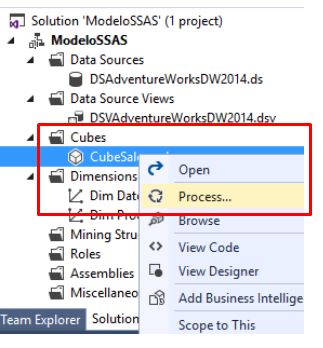
\includegraphics[width=8cm]{images/task4/img22}
	\end{center}	
	Click en Yes
	\begin{center}
	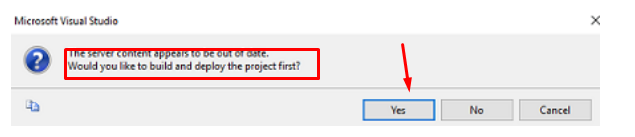
\includegraphics[width=8cm]{images/task4/img23}
	\end{center}	
En la nueva ventana seleccionamos la opción de Run…
	\begin{center}
	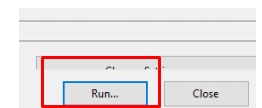
\includegraphics[width=8cm]{images/task4/img24}
	\end{center}	
Si todo va bien nos mostrará algo como lo siguiente:
	\begin{center}
	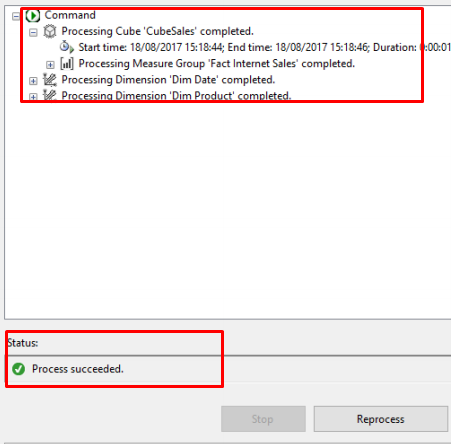
\includegraphics[width=8cm]{images/task4/img25}
	\end{center}	
Para verificar que nuestros datos se procesaron de forma correcta , en el cubo CubeSales nos dirigimos a la
pestaña de Browse:
	\begin{center}
	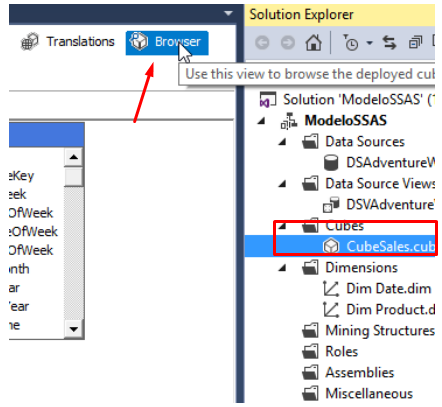
\includegraphics[width=8cm]{images/task4/img26}
	\end{center}	
En la pestaña de CubeSales, podemos tener un vistazo de las medidas y dimensiones. Arrastramos las
columnas de la Fact y la Dimensión Product obteniendo algo como:
	\begin{center}
	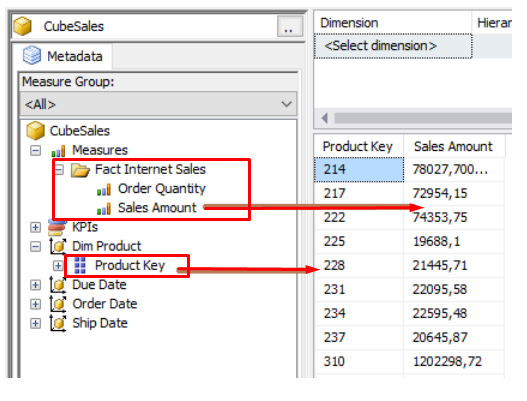
\includegraphics[width=8cm]{images/task4/img27}
	\end{center}	